\begin{figure}[ht!]
    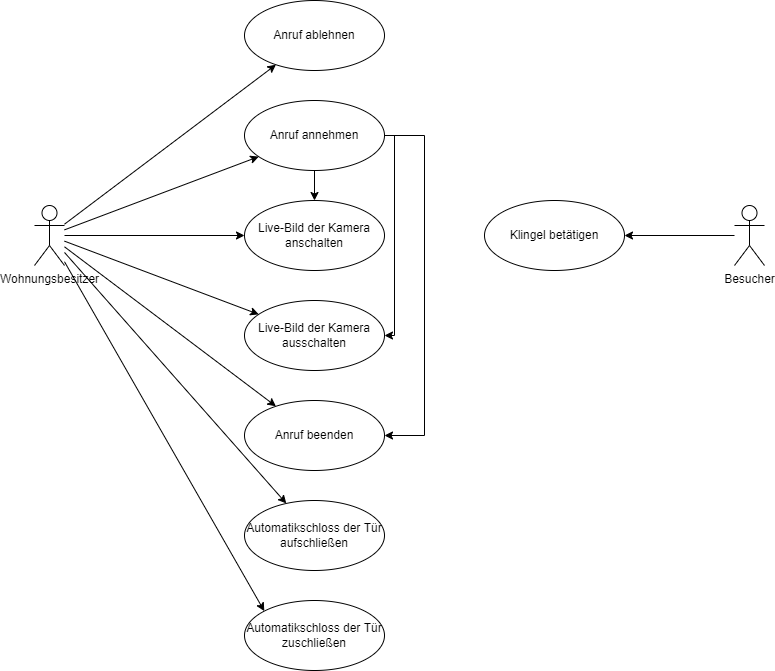
\includegraphics[width=\paperwidth-2in]{../assets/img/UML-Anwendungsfalldiagramme-Klingeln bei einem Mehrfamilienhaus}
    \caption{Diagram}
    \label{fig:diagram}
\end{figure}


\paragraph{Klingel betätigen}
    \begin{description}
        \item[Ziel]\hfill \\
        Besucher möchte klingeln.
        \item[Beschreibung]\hfill \\
        Klingel wird betätigt, um Kontakt zu Wohnungsbesitzer aufzunehmen.
        \item[Akteure]\hfill \\
        Besucher.
        \item[Auslöser]\hfill \\
        Besucher möchte Kontakt zu Wohnungsbesitzer aufnehmen..
        \item[Vorbedingungen]\hfill \\
        Keine.
        \item[Nachbedingungen]\hfill \\
        Wohnungsbesitzer wird angerufen.
        \end{description}

\paragraph{Anruf annehmen}
    \begin{description}
        \item[Ziel]\hfill \\
        Ein eingehender Anruf soll angenommen werden.
        \item[Beschreibung]\hfill \\
        Indem der Benutzer auf die eingehende Bena
        \item chrichtigung klickt, wird der Anruf angenommen.
        Wenn die Visualisierung beim Benutzer schon geöffnet ist, kann der Anruf auch in der Visualisierung angenommen werden.
        \item[Akteure]\hfill \\
        Wohnungsbesitzer, Reparatur-Mitarbeiter, Zimmerservice.
        \item[Auslöser]\hfill \\
        Eingehender Anruf.
        \item[Vorbedingungen]\hfill \\
        Besucher hat Klingel betätigt oder Industrie-Mitarbeiter oder Hotelgast hat Kontakt angerufen.
        \item[Nachbedingungen]\hfill \\
        Anruf wurde angenommen und Gespräch gestartet.
        \end{description}

\paragraph{Anruf ablehnen}
    \begin{description}
        \item[Ziel]\hfill \\
        Ein eingehender Anruf soll abgelehnt werden.
        \item[Beschreibung]\hfill \\
        Indem der Benutzer die eingehende Benachritigung wegklickt, wird der Anruf abgelehnt.
        Wenn die Visualisierung beim Benutzer schon geöffnet ist, kann der Anruf auch in der Visualisierung abgelehnt werden.
        \item[Akteure]\hfill \\
        Wohnungsbesitzer, Reparatur-Mitarbeiter, Zimmerservice.
        \item[Auslöser]\hfill \\
        Eingehender Anruf.
        \item[Vorbedingungen]\hfill \\
        Besucher hat Klingel betätigt oder Industrie-Mitarbeiter oder Hotelgast hat Kontakt angerufen.
        \item[Nachbedingungen]\hfill \\
        Anruf wurde abgelehnt.
        \end{description}

\paragraph{Anruf beenden}
    \begin{description}
        \item[Ziel]\hfill \\
        Ein laufender Anruf soll beendet werden.
        \item[Beschreibung]\hfill \\
        Indem der Benutzer in der Visualisierung den Button zum Auflegen betätigt, kann der Anruf jederzeit beendet werden.
        \item[Akteure]\hfill \\
        Wohnungsbesitzer, Industrie-Mitarbeiter, Reparatur-Mitarbeiter, Hotelgast, Zimmerservice.
        \item[Auslöser]\hfill \\
        Einer der Akteure möchte den Anruf beenden.
        \item[Vorbedingungen]\hfill \\
        Wohnungsbesitzer, Reparatur-Mitarbeiter oder Zimmerservice hat einen Anruf angenommen.
        \item[Nachbedingungen]\hfill \\
        Anruf wurde beendet.
        \end{description}

\paragraph{Anruf weiterleiten}
    \begin{description}
        \item[Ziel]\hfill \\
        Ein eingehender Anruf soll an einen ausgewählten Kontakt weitergeleitet werden.
        \item[Beschreibung]\hfill \\
        Indem der Benutzer in der Visualisierung den Button zum Weiterleiten betätigt, kann der eingehende Anruf an einen verfügbaren Kontakt weitergeleitet werden.
        Diesen Kontakt kann er anschließend wie im Anwendungsfall "Kontakt suchen und auswählen" wählen.
        Mit einem weiteren Knopfdruck wird der Anruf an den ausgewählten Kontakt weitergeleitet.
        \item[Akteure]\hfill \\
        Reparatur-Mitarbeiter.
        \item[Auslöser]\hfill \\
        Eingehender Anruf.
        \item[Vorbedingungen]\hfill \\
        Industrie-Mitarbeiter hat Kontakt des Reparatur-Unternehmens angerufen.
        \item[Nachbedingungen]\hfill \\
        Anruf wurde an ausgewählten Kontakt weitergeleitet.
        \end{description}

\paragraph{Live-Bild der Kamera anschalten}
    \begin{description}
        \item[Ziel]\hfill \\
        Das Live-Bild der Kamera an der Eingangstür soll angeschaltet werden.
        \item[Beschreibung]\hfill \\
        Indem der Benutzer in der Visualisierung den entsprechenden Button betätigt, wird das Live-Bild angeschaltet.
        \item[Akteure]\hfill \\
        Wohnungsbesitzer.
        \item[Auslöser]\hfill \\
        Der Wohnungsbesitzer möchte das Live-Bild der Kamera sehen.
        \item[Vorbedingungen]\hfill \\
        Besucher hat Klingel betätigt und Wohnungsbesitzer hat den daraufhin ausgelösten Anruf angenommen.
        Das Live-Bild ist ausgeschaltet.
        \item[Nachbedingungen]\hfill \\
        Live-Bild wurde für den Wohnungsbesitzer angeschaltet.
        \end{description}

\paragraph{Live-Bild der Kamera ausschalten}
    \begin{description}
        \item[Ziel]\hfill \\
        Das Live-Bild der Kamera an der Eingangstür soll ausgeschaltet werden.
        \item[Beschreibung]\hfill \\
        Indem der Benutzer in der Visualisierung den entsprechenden Button betätigt, wird das Live-Bild ausgeschaltet.
        \item[Akteure]\hfill \\
        Wohnungsbesitzer.
        \item[Auslöser]\hfill \\
        Der Wohnungsbesitzer möchte das Live-Bild der Kamera nicht mehr sehen.
        \item[Vorbedingungen]\hfill \\
        Besucher hat Klingel betätigt und Wohnungsbesitzer hat den daraufhin ausgelösten Anruf angenommen.
        Das Live-Bild ist angeschaltet.
        \item[Nachbedingungen]\hfill \\
        Live-Bild wurde für den Wohnungsbesitzer ausgeschaltet.
        \end{description}

\paragraph{Automatikschloss der Tür aufschließen}
    \begin{description}
        \item[Ziel]\hfill \\
        Das Automatikschloss der Eingangstür soll aufgeschlossen werden, um den Besucher ins Gebäude zu lassen.
        \item[Beschreibung]\hfill \\
        Indem der Benutzer in der Visualisierung den entsprechenden Button betätigt, wird das Automatikschloss aufgeschlossen.
        \item[Akteure]\hfill \\
        Wohnungsbesitzer.
        \item[Auslöser]\hfill \\
        Der Wohnungsbesitzer möchte den Besucher ins Gebäude lassen.
        \item[Vorbedingungen]\hfill \\
        Besucher hat Klingel betätigt und Wohnungsbesitzer hat den daraufhin ausgelösten Anruf angenommen.
        \item[Nachbedingungen]\hfill \\
        Das Automatikschloss der Eingangstür wurde aufgeschlossen.
        \end{description}

\paragraph{Automatikschloss der Tür zuschließen}
    \begin{description}
        \item[Ziel]\hfill \\
        Das Automatikschloss der Eingangstür soll zugeschlossen werden.
        \item[Beschreibung]\hfill \\
        Indem der Benutzer in der Visualisierung den entsprechenden Button betätigt, wird das Automatikschloss zugeschlossen.
        \item[Akteure]\hfill \\
        Wohnungsbesitzer.
        \item[Auslöser]\hfill \\
        Der Wohnungsbesitzer möchte die Eingangstür zuschließen.
        \item[Vorbedingungen]\hfill \\
        Besucher hat Klingel betätigt und Wohnungsbesitzer hat den daraufhin ausgelösten Anruf angenommen.
        \item[Nachbedingungen]\hfill \\
        Das Automatikschloss der Eingangstür wurde zugeschlossen.
        \end{description}

\paragraph{Kontakt suchen und auswählen}
    \begin{description}
        \item[Ziel]\hfill \\
        Der Benutzer hat einen gesuchten Kontakt ausgewählt, wenn es ihn gibt.
        \item[Beschreibung]\hfill \\
        Über eine Liste in der Visualisierung, eventuell auch Favoritenliste, kann der Benutzer einen Kontakt auswählen.
        Er kann auch einen Kontakt über eine Suchleiste suchen und diesen auswählen, wenn es ihn gibt.
        \item[Akteure]\hfill \\
        Industrie-Mitarbeiter, Hotelgast.
        \item[Auslöser]\hfill \\
        Benutzer möchte Kontakt finden.
        \item[Vorbedingungen]\hfill \\
        Keine.
        \item[Nachbedingungen]\hfill \\
        Keine oder ein Kontakt wurde ausgewählt und kann angerufen werden.
        \end{description}

\paragraph{Kontakt anrufen}
    \begin{description}
        \item[Ziel]\hfill \\
        Der Benutzer startet einen Anruf mit dem ausgewählten Kontakt.
        \item[Beschreibung]\hfill \\
        Hat der Benutzer einen Kontakt ausgewählt, kann er diesen über einen Button anrufen.
        \item[Akteure]\hfill \\
        Industrie-Mitarbeiter, Hotelgast.
        \item[Auslöser]\hfill \\
        Benutzer möchte Kontakt anrufen.
        \item[Vorbedingungen]\hfill \\
        Ein Kontakt wurde ausgewählt.
        \item[Nachbedingungen]\hfill \\
        Ein Anruf mit Kontakt wurde gestartet.
        \end{description}

\paragraph{Bildschirmfreigabe starten}
    \begin{description}
        \item[Ziel]\hfill \\
        Die Bildschirmfreigabe soll gestartet werden.
        \item[Beschreibung]\hfill \\
        Indem der Benutzer in der Visualisierung den entsprechenden Button betätigt, wird sein Bildschirm mit dem anderen Teilnehmer des Anrufs geteilt.
        \item[Akteure]\hfill \\
        Industrie-Mitarbeiter.
        \item[Auslöser]\hfill \\
        Der Industrie-Mitarbeiter möchte seinen Bildschirm mit dem Reparatur-Mitarbeiter teilen.
        \item[Vorbedingungen]\hfill \\
        Reparatur-Mitarbeiter hat einen Anruf angenommen.
        Es wurde noch keine Bildschirmfreigabe gestartet oder diese wurde schon wieder gestoppt.
        \item[Nachbedingungen]\hfill \\
        Die Bildschirmfreigabe wurde gestartet.
        \end{description}

\paragraph{Bildschirmfreigabe stoppen}
    \begin{description}
        \item[Ziel]\hfill \\
        Die Bildschirmfreigabe soll gestoppt werden.
        \item[Beschreibung]\hfill \\
        Indem der Benutzer in der Visualisierung den entsprechenden Button betätigt, wird das Teilen seines Bildschirms mit dem anderen Teilnehmer des Anrufs gestoppt.
        \item[Akteure]\hfill \\
        Industrie-Mitarbeiter.
        \item[Auslöser]\hfill \\
        Der Industrie-Mitarbeiter möchte seinen Bildschirm nicht mehr mit dem Reparatur-Mitarbeiter teilen.
        \item[Vorbedingungen]\hfill \\
        Reparatur-Mitarbeiter hat einen Anruf angenommen.
        Die Bildschirmfreigabe wurde gestartet.
        \item[Nachbedingungen]\hfill \\
        Die Bildschirmfreigabe wurde gestoppt.
        \end{description}

\paragraph{Aufgezeichnetes Videomaterial einsehen}
    \begin{description}
        \item[Ziel]\hfill \\
        Aufgezeichnetes Videomaterial, das nicht älter als eine Woche ist, soll eingesehen werden.
        \item[Beschreibung]\hfill \\
        Über die Visualisierung kann der Benutzer, über eine Liste, die Kamera auswählen, von der er das aufgezeichnete Videomaterial einsehen möchte.
        Darufhin wird ihm das entsprechende Videomaterial der letzten 7 Tage angezeigt.
        \item[Akteure]\hfill \\
        Hausverwalter.
        \item[Auslöser]\hfill \\
        Hausverwalter möchte Videomaterial einsehen.
        \item[Vorbedingungen]\hfill \\
        Keine.
        \item[Nachbedingungen]\hfill \\
        Aufgezeichnetes Videomaterial, das nicht älter als eine Woche ist, wurde eingesehen.
        \end{description}   